\section{\scshape Recognition System}\label{sec:methodology}

\subsection{Recognition System Overview}
\begin{frame}{Recognition System Overview}
	\begin{figure}
		\centering
		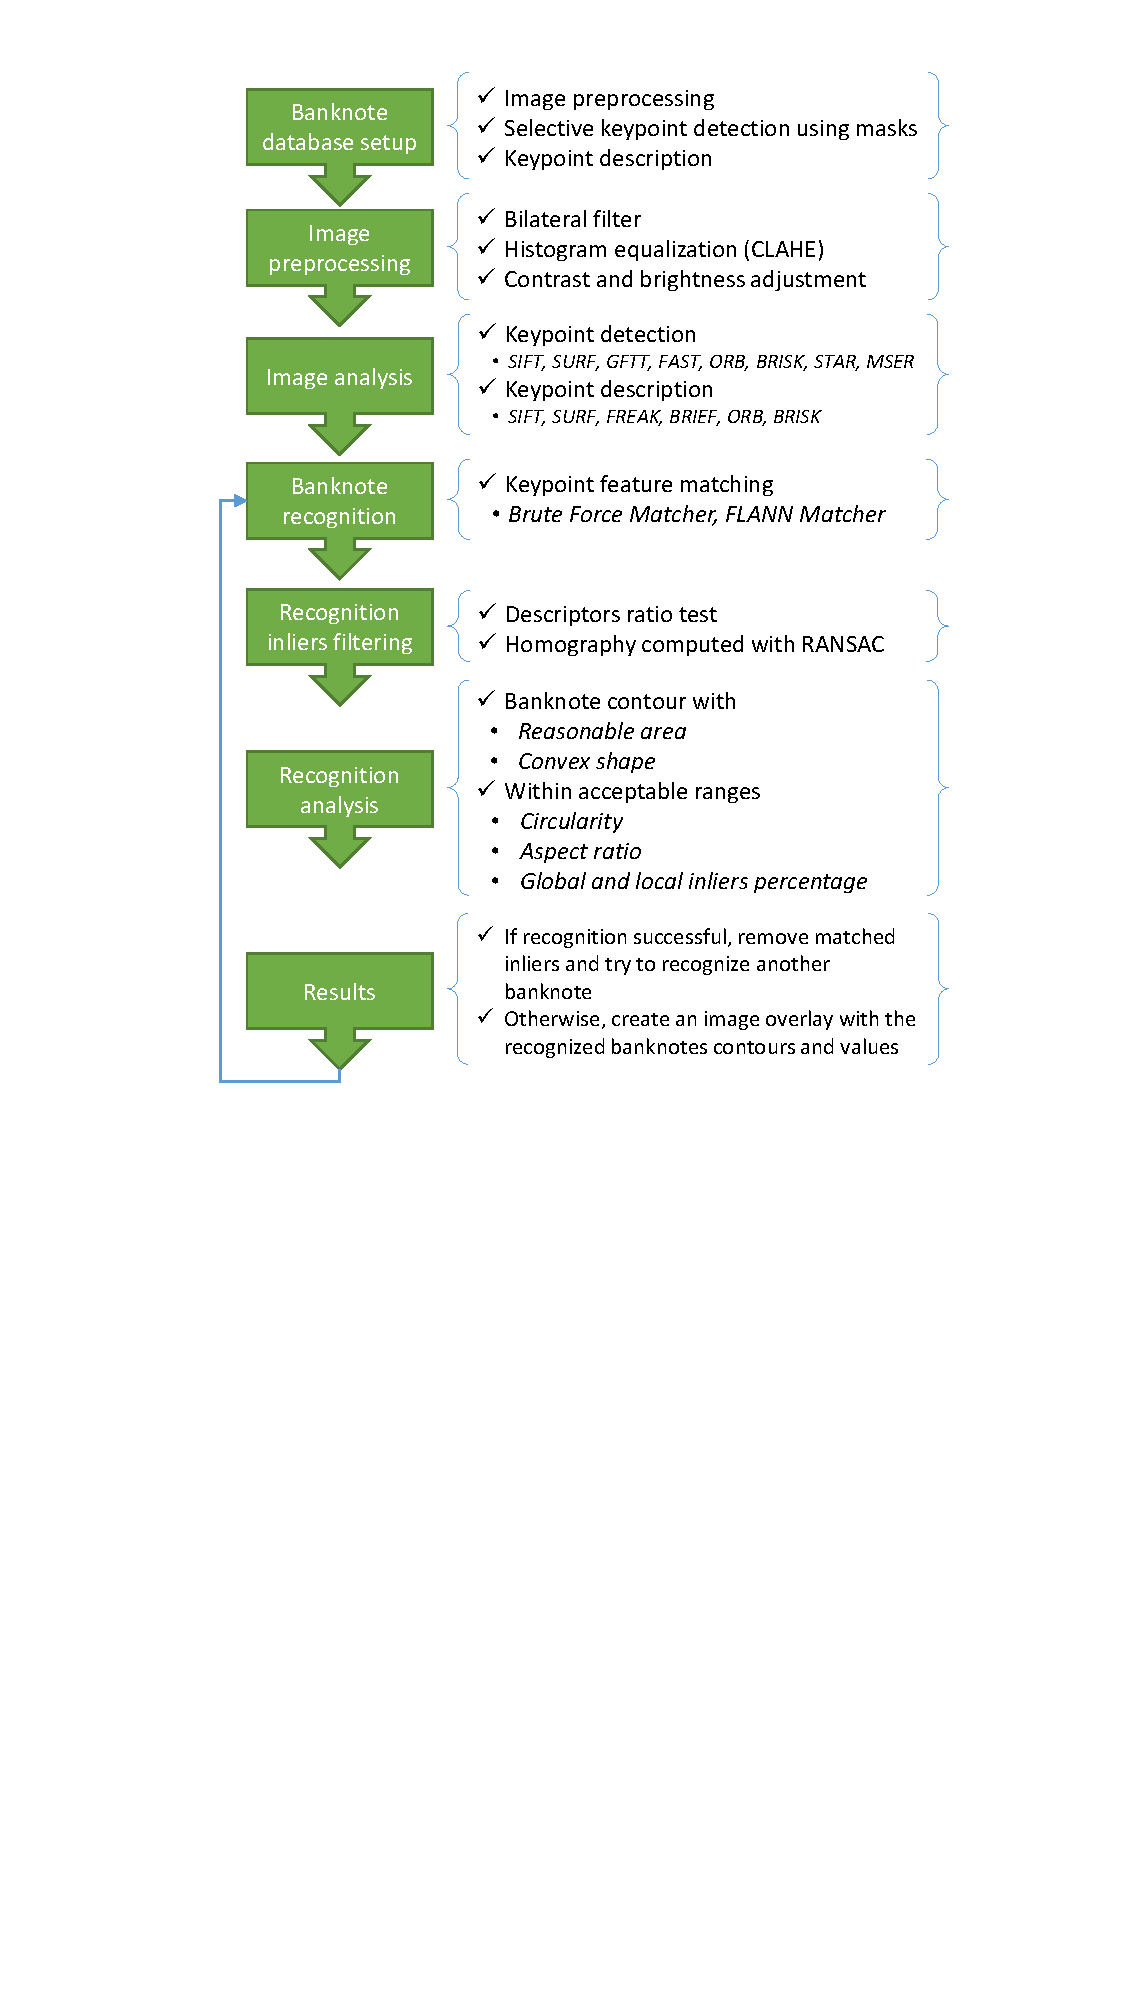
\includegraphics[width=0.52\linewidth]{system-overview}
		\label{fig:system-overview}
	\end{figure}
\end{frame}


\subsection{Banknote Database Setup}
\begin{frame}{Banknote Database Setup}
	\begin{itemize}
		\item Multi-resolution recognition database
		\begin{itemize}
			\item Image width of 256, 512 and 1024 pixels
		\end{itemize}
		
		\item Each banknote is subjected to
		\begin{itemize}
			\item Image preprocessing
			\item Selective keypoint detection using masks
			\item Keypoint description
		\end{itemize}
	\end{itemize}
	
	\begin{figure}[H]
		\centering
		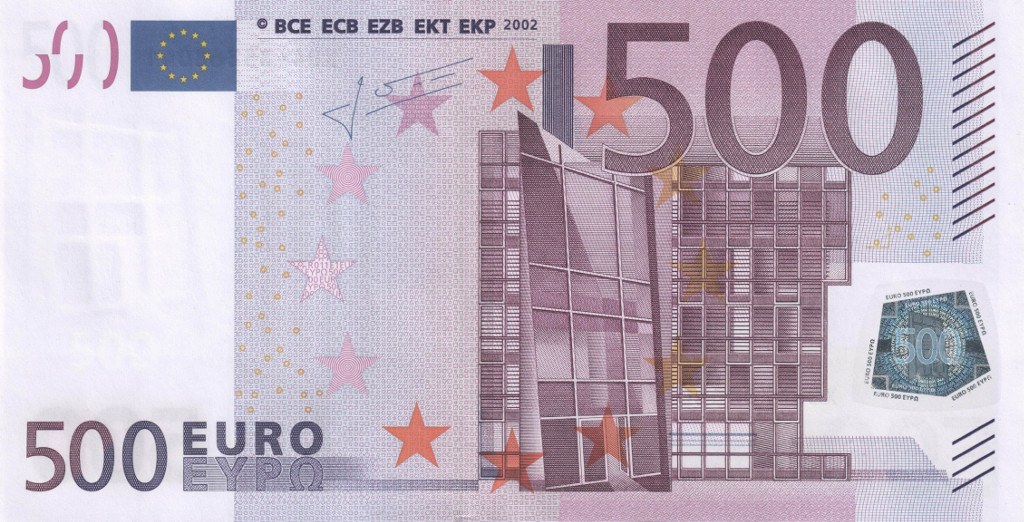
\includegraphics[width=.33\textwidth]{notes-masks/500eu-front}
		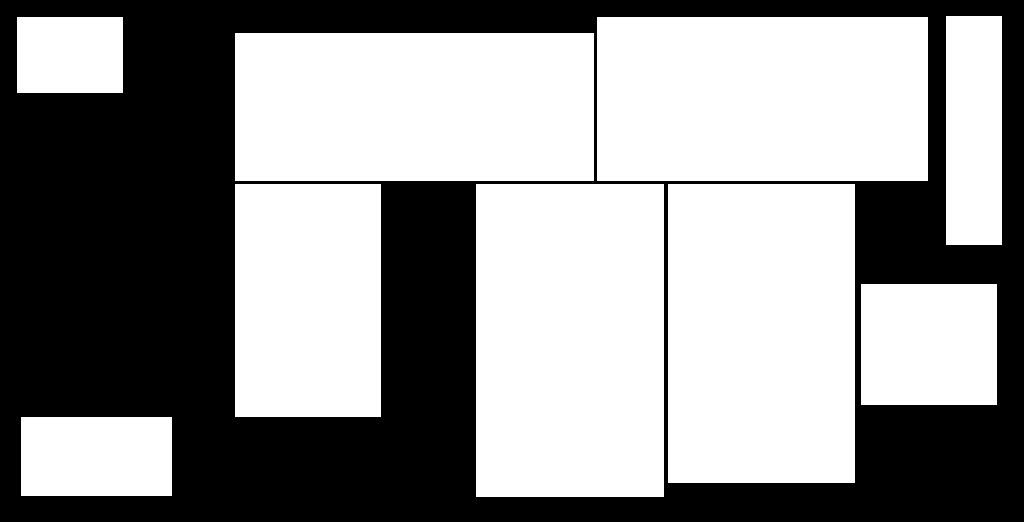
\includegraphics[width=.33\textwidth]{notes-masks/500eu-front-mask}\\
		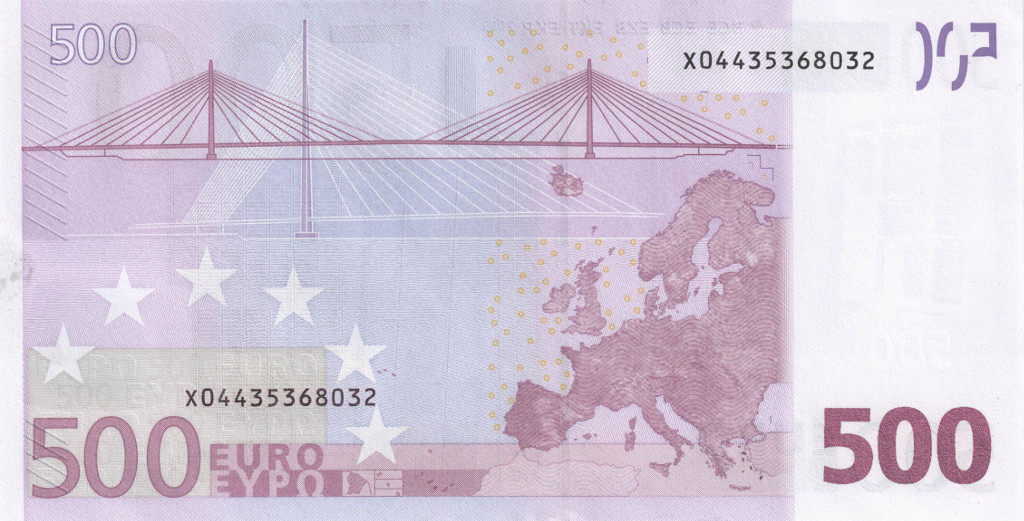
\includegraphics[width=.33\textwidth]{notes-masks/500eu-back}
		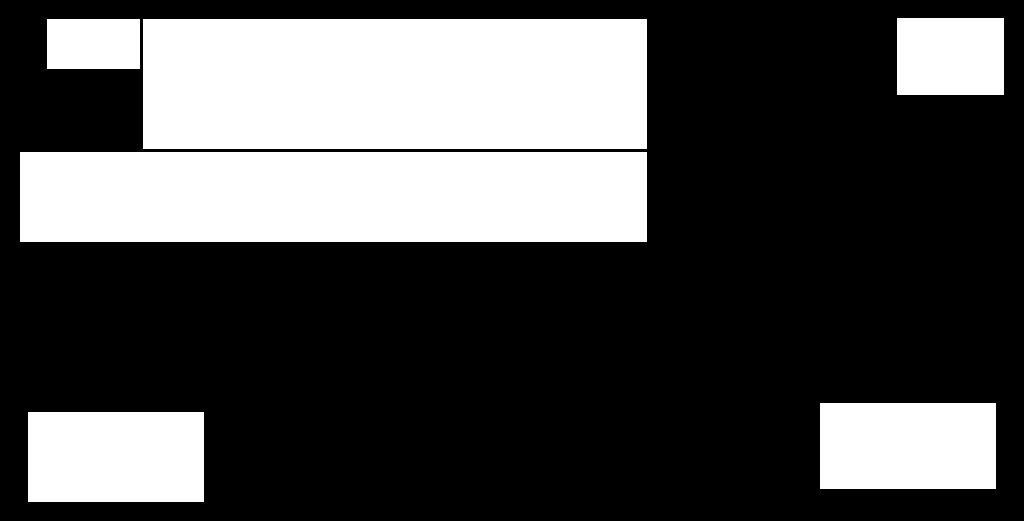
\includegraphics[width=.33\textwidth]{notes-masks/500eu-back-mask}
		\caption{Front and back of a 500\,\euro{} banknote with associated feature detection masks}
		\label{fig:banknote-feature-detection-mask-500-front}
	\end{figure}
\end{frame}


\subsection{Image Preprocessing}
\begin{frame}{Image Preprocessing}
	\begin{itemize}
		\item Bilateral filter
		\item Contrast Limited Adaptive Histogram Equalization
		\item Contrast and brightness tunning
	\end{itemize}
	
	\begin{figure}[H]
		\centering
		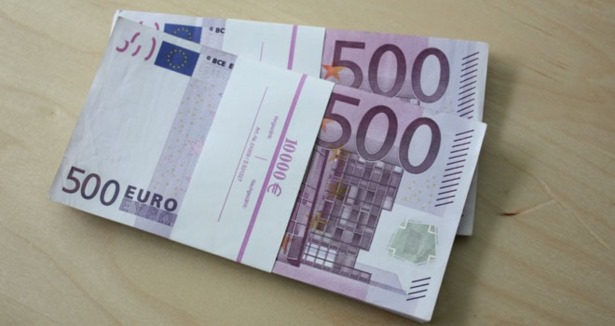
\includegraphics[width=.4\textwidth]{preprocessing/500-500}
		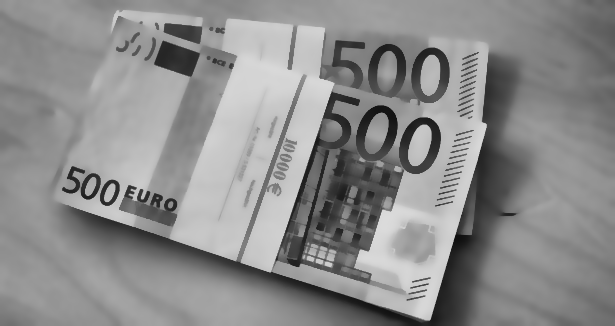
\includegraphics[width=.4\textwidth]{preprocessing/500-500-preprocessed}\\
		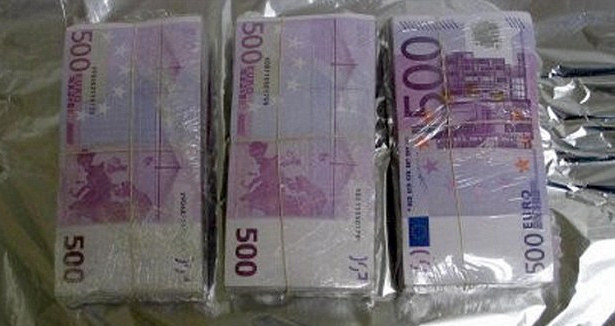
\includegraphics[width=.4\textwidth]{preprocessing/500-500-500}
		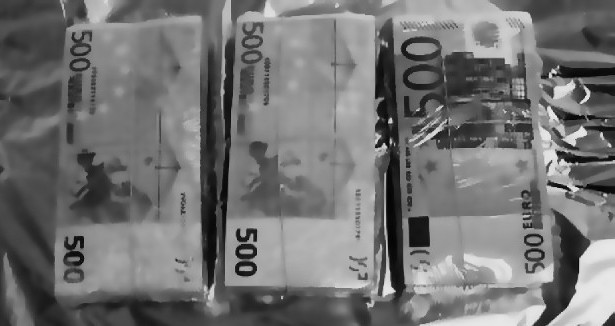
\includegraphics[width=.4\textwidth]{preprocessing/500-500-500-preprocessed}
		\caption{Impact of preprocessing stage on two pairs of images (original image on the left, preprocessed image on the right)}
		\label{fig:preprocessing}
	\end{figure}
\end{frame}


\subsection{Image Analysis}
\begin{frame}{Image Analysis}
	\begin{itemize}
		\item Keypoint detection
		\begin{itemize}
			\item SIFT, SURF, GFTT, FAST, ORB, BRISK, STAR, MSER
		\end{itemize}
		\item Keypoint description
		\begin{itemize}
			\item SIFT, SURF, FREAK, BRIEF, ORB, BRISK
		\end{itemize}
	\end{itemize}
	
	\begin{figure}[H]
		\centering
		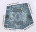
\includegraphics[width=.2496\textwidth]{image-resolution/500eu-front-very-low}\hfill
		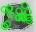
\includegraphics[width=.2496\textwidth]{image-resolution/500eu_front_currencyDB_veryLowResolution_SIFT-Detector}\hfill
		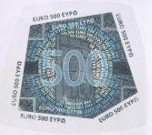
\includegraphics[width=.2499\textwidth]{image-resolution/500eu-front-medium}\hfill
		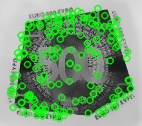
\includegraphics[width=.2499\textwidth]{image-resolution/500eu_front_currencyDB_mediumResolution_SIFT-Detector}
		\caption{Impact of image resolution when computing SIFT keypoints from a very low resolution image (left) to a high resolution image (right) of the hologram of a 500\,\euro{} banknote}
		\label{fig:banknote-500-front-resolution-difference}
	\end{figure}
\end{frame}


\subsection{Banknote Recognition}
\begin{frame}{Banknote Recognition}
	\begin{itemize}
		\item Keypoint feature matching
		\begin{itemize}
			\item Brute Force Matcher, FLANN Matcher
		\end{itemize}
	\end{itemize}

	\begin{figure}[H]
		\centering
		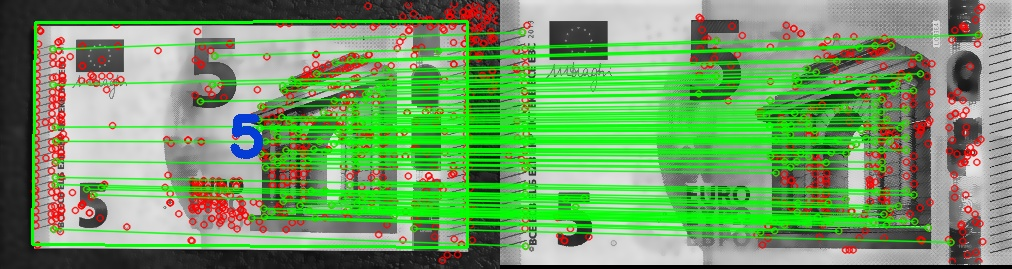
\includegraphics[width=\textwidth]{notes-recognition/5__(5).jpg___SIFT-Detector_SIFT-Extractor_BF-Matcher_lowQualityImageDB_globalMatch__inliersMatches__0}
		\caption{Feature matching on a banknote in an ideal perspective view (using SIFT detector, SIFT descriptors and BFMatcher)}
		\label{fig:recognition-front}
	\end{figure}
\end{frame}


\subsection{Recognition Analysis}
\begin{frame}{Recognition Analysis}
	\begin{itemize}
		\item Recognition inliers filtering using
		\begin{itemize}
			\item Matched descriptors ratio test
			\item Homography computed with RANSAC
		\end{itemize}
		
		\item Banknote contour with
		\begin{itemize}
			\item Reasonable area
			\item Convex shape
		\end{itemize}
		
		\item Within acceptable ranges
		\begin{itemize}
			\item Circularity
			\item Aspect ratio
			\item Global and local (mask patch) inliers percentage
		\end{itemize}
	\end{itemize}

	\begin{figure}
		\centering
		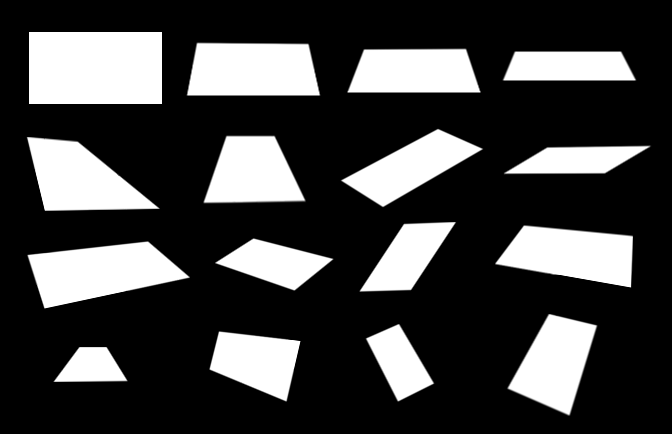
\includegraphics[width=0.35\textwidth]{notes-masks/currency-db-shapes}
		\caption{Database of valid instances of banknote shapes}
		\label{fig:currency-db-shapes}
	\end{figure}
\end{frame}


\subsection{Recognition Output Overlay}
\begin{frame}{Recognition Output Overlay}
	\begin{itemize}
		\item If recognition successful, matched inliers are removed and the system tries to recognize another banknote
		\item Otherwise it is created an image overlay with the recognized banknotes contours and values
	\end{itemize}
	\begin{figure}[H]
		\centering
		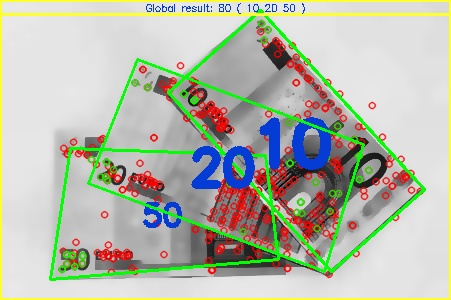
\includegraphics[width=0.6\textwidth]{notes-recognition/10-20-50.jpg___SIFT-Detector_SIFT-Extractor_BF-Matcher_dynamicQualityImageDB_globalMatch}
		\caption{Image overlay containing the recognized banknotes values and contours (used SIFT detector, SIFT descriptors and BFMatcher)}
		\label{fig:recognition-overlapping-banknotes-0}
	\end{figure}
\end{frame}
